\chapter{Materiais e Métodos} \label{cap:metod}

Nesse capítulo são descritos os métodos, assim como os materiais utilizados para o desenvolvimento deste trabalho. São descritas as etapas do projeto e os principais fundamentos e tecnologias a serem empregados.


\section{Materiais}
% arnaldo: 3.1 materiais: flutter, dart, python, mlkit, firebase, macbook para codificar (processador, memória, ...), software de emulação, iphone (geração, câmera, ...)
O ambiente de desenvolvimento da metodologia proposta se faz o uso de um Macbook Pro de 13 polegadas com processador Intel Core i5 de dois núcleos 2,3 GHz e memória integrada LPDDR3 de 8 GB com 2133 MHz e embarcado com o sistema operacional macOS Mojave versão 10.14.4.  

Para o desenvolvimento da metodologia, foi optado por utilizar as tecnologias de aplicativos móveis como Flutter, Dart e Firebase MLKit devido às suas altas taxas de aprendizado e desempenho no desenvolvimento de aplicativos móveis.

O Flutter\footnote{https://flutter.dev/} foi construído pela Google com a finalidade de melhorar a qualidade dos aplicativos, a velocidade do desenvolvimento, e para alcançar mais usuários. Ele é um SDK  de código aberto para o desenvolvimento de aplicativos para Desktop, Web e dispositivos móveis como iOS e Android \cite{ARSTECHNICA2017}.


O Flutter é um poderoso \texttit{framework} porque o código é compilado em ARM, ou seja, compila o código para cada plataforma. Isso agiliza a abertura e o desempenho do aplicativo. Além disso, utiliza um renderizador Mobile First acelerado por GPU para que haja consistência da \texttit{UI} entre as plataformas e o dispositivo. Então o Flutter projeta os \texttit{widgets} com um \texttit{framework} personalizável e extensível em camadas \cite{IMASTERS}. Não há pontes entre o \texttit{framerwork} e os \texttit{widgets}, tornando a renderização eficiente. 

Flutter é escrito em Dart, uma linguagem concisa, fortemente tipificada e orientada a objetos. O Dart é bem semelhante à linguagens como Swift, C#, Java e JavaScript.



Para a extração dos caracteres da imagem será utilizado o SDK Firebase ML Kit\footnote{https://firebase.google.com/}, após a etapa de pré-processamento será testado a eficácia tanto da sua versão \texttit{online} quanto \texttit{offline}, para uma taxa maior de acertos nas palavras, diminuindo a complexidade da busca pelos registros na base de dados da ANVISA, disponibilizada em seu \texttit{site} oficial.

Os testes serão realizados por meio de um dispositivo físico, Samsung J2 com processador de 1.4GHz, equipado com câmera traseira com resolução de 8.0 MP  e um iPhone 7, equipado com uma câmera de 12 MP com resolução de 1334x750 pixeis e abertura de abertura de ƒ/1.8, processador Quad-Core 2 GHZ, armazenamento de 128 GB e com sistema operacional iOS na versão 12.2.



% arnaldo: 3.2 método: criar base (capturar imagens, dizer quantas imagens,  resolução, colorido, iluminação);  pré-processar para tirar as bordas e corrigir a perspectiva; ocr; buscar na base; vai ter algum pos-processamento (ex. corretor ortográfico para contorar falhas do ocr)


\section{Coleta de imagens}

Foi necesário ser feita a coleta de caixas de medicamentos para formar a base de imagens. Foram coletadas 6 caixas de medicamentos conforme a Figura \ref{exemplares}, com especificações diferentes, entre elas: proporções, fontes, cores e finalidade. Entre as caixas de medicamento, apenas um medicamento entre os 6 não é regulamentarizado pela a Anvisa, o que foi um ponto importante para o desenvolvimento do aplicativo. Todas as caixas coletadas foram fornecidas pela farmácia Hiper Farma da cidade de Medianeira. Dessa manaeira, foi possível ser construído a base de imagens.

 \begin{figure}[h!]
	\centering
	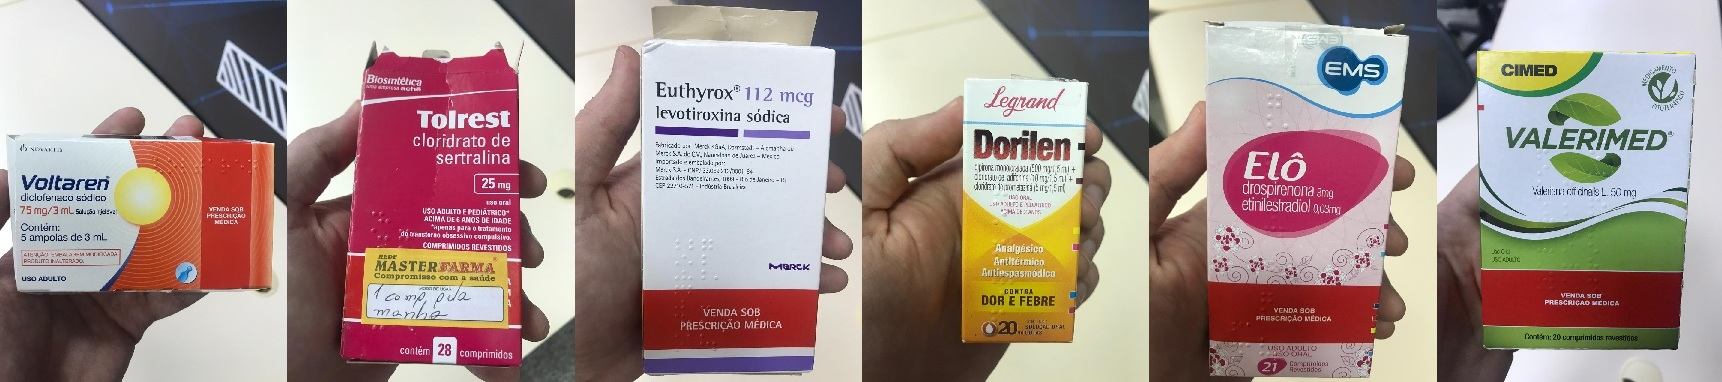
\includegraphics[width=0.99\textwidth]{Imagens/exemplares.jpg} 
	\caption[Exemplares de medicamentos utilizados.]{Exemplares de medicamentos utilizados.}
\fonte{Autoria própria.}
	\label{exemplares}
\end{figure}


A base de imagens composta por 150 imagens com resolução de 3264x2448 \textit{pixel}, classificadas em 5 categorias: 

  \begin{enumerate}
   \item Fotos em ambiente com boa luminosidade.
   \item Fotos em ambiente com baixa luminosidade.
   \item Fotos expostas ao ambiente externo no sol.
   \item Fotos noturnas sem flash.
   \item Fotos noturnas com flash.
 \end{enumerate}
 
\subsection{Categorias da base de imagens}

 Todas as categorias são compostas por imagens de 6 medicamentos, onde cada medicamento possui 5 fotos em cada categoria. Cada foto foi capturada em uma diferente perspectiva, formando assim, 5 perspectivas demonstradas na Figura \ref{perspectiva}, que são:
   \begin{enumerate}
   \item Fotos chapadas, com a captura perpendicular ao plano de interesse da caixa.
   \item Fotos do topo, com inclinação média de 15 graus no topo em relação ao plano de interesse da caixa.
    \item Fotos da lateral esquerda, com inclinação aproximada de 15 graus na lateral esquerda em relação ao plano de interesse da caixa.
    \item Fotos da lateral direita, com inclinação média de 15 graus na lateral direita em relação ao plano de interesse da caixa.
    \item Fotos da base inferior, com inclinação média de 15 graus na base inferior em relação ao plano de interesse da caixa.
 \end{enumerate}
  \begin{figure}[h!]
	\centering
	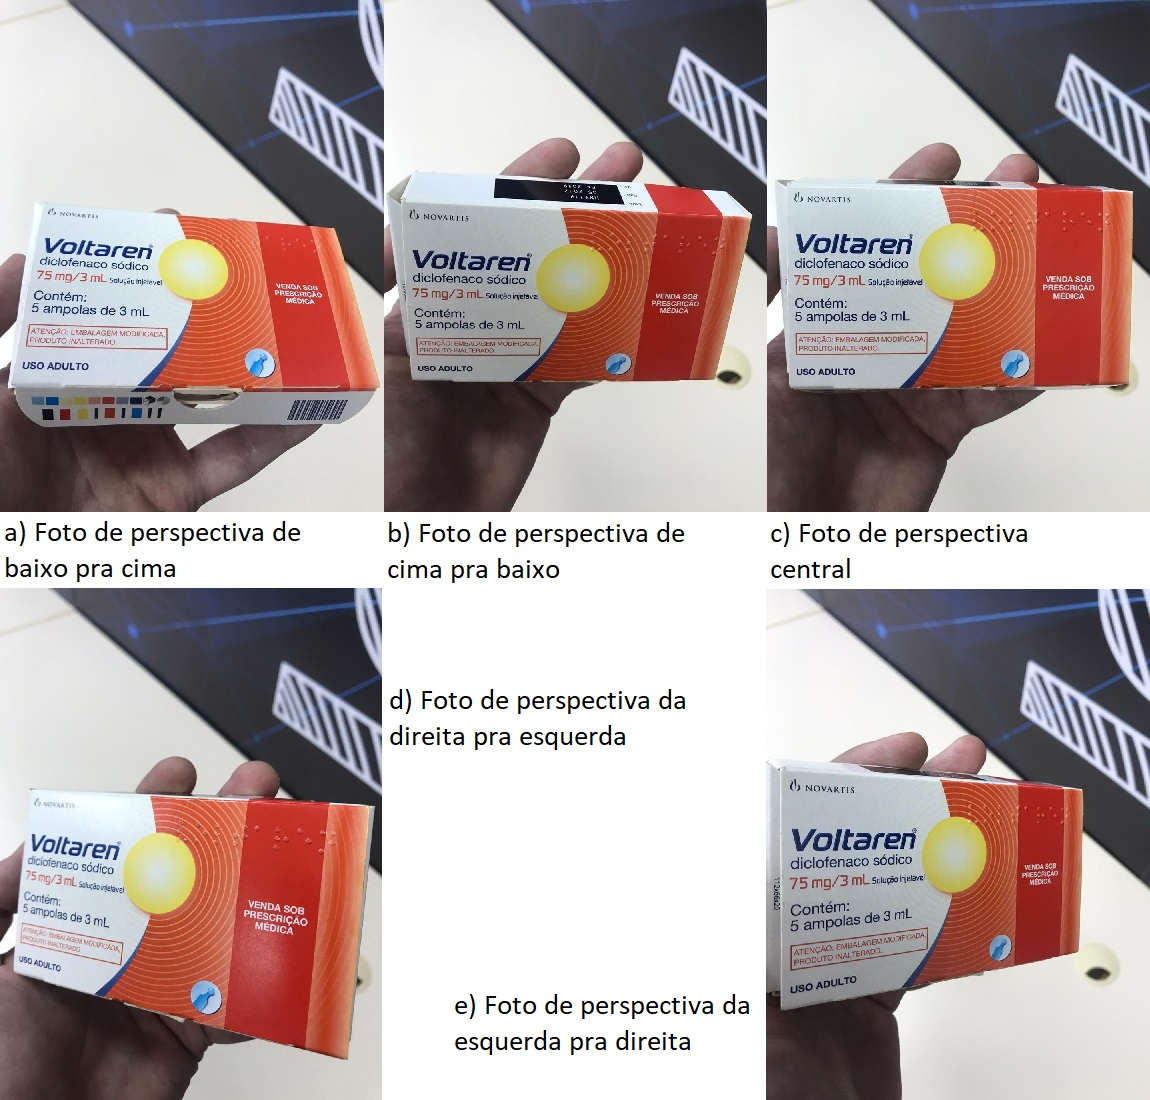
\includegraphics[height=0.70\textwidth]{Imagens/perspectiva.jpg} 
	\caption[Exemplar de medicamento em diferentes perspectivas.]{Exemplar de medicamento em diferentes perspectivas}
\fonte{Autoria própria.}
	\label{perspectiva}
\end{figure}
 
 
 No decorrer da criação da base de imagens, foi constatado que o dispositivo celular Samsung J2 
 não possui boa captura de imagens em ambientes com baixa luminosidade, mas ainda assim optou-se por realizar a captura e os testes, pelo fato de reproduzir uma situação remota e existente no cotidiano dos brasileiros.


\section{Desenvolvimento do aplicativo}
Inicialmente, os aplicativos criados nesse trabalho foram desenvolvidos fazendo uso do \textit{framework} Flutter, como previstos na sessão de materiais. A versão utilizada para os experimentos foram as versões 1.9 do Flutter e 2.5 do Dart (linguagem utilizada pelo Flutter). O ambiente para o desenvolvimento foi \textit{Windows 10 64 bits} e a ferramenta específica para a implementação foi a \textit{IDE} Android Studio versão 3.5.
Os testes de execução da aplicação ocorreu em um dispositivo celular  modelo Samsung J2 Prime, portando um processador de 1.4 \textit{GHz Quad Core} e uma câmera traseira de 8 \textit{megapixel}. 

Para a configuração do plugin que faz uso do OCR, foi utilizado o framework Firebase MLKit para o reconhecimento de caracteres. Este framework possui recursos para reconhecimento de imagens
\textit{online} e \textit{offline},
que permite ser feita a comparação do reconhecedor de caracteres, tanto online no servidor do \textit{framework}, quanto \textit{offline} no dispositivo.

O pacote de desenvolvimento do \textit{Firebase ML Vision} foi utilizado na versão 0.9.2, lançada em 23 de julho de 2019.	Utilizando o pacote de desenvolvimento do \textit{Firebase Vision}, é possível extrair o texto em 3 diferentes formas: em blocos, linha e palavras, todas com seu nível de confiança de 0 a 100 porcento, onde 0 porcento indica não confiável ao poder acertivo do OCR e 100 porcento significa total certeza de poder acertivo do OCR.
 
 Para armazenar os dados dos medicamentos extraídos do bulário da Anvisa, foi configurado um banco de dados \textit{SQLite} na versão 1.1.6, lançada em 25 junho de 2019. 


% Com a imagem já tratada, a última etapa do pré-processamento é o recorte da área de interesse já corrigida, substituindo a imagem original, para a extração de texto no OCR.

% Após o reconhecimento dos caracteres, é possível que necessite a utilização de um corretor ortográfico para contornar falhas de reconhecimento do OCR. Será testado a eficácia do corretor ortográfico do Firebase ML Kit, que é um dicionário latino brasileiro. Caso o mesmo não venha atender as expectativas de contorno de falhas do OCR, será estudado outra opção de corretor ortográfico.

% Para finalizar, as palavras encontradas estarão prontas para serem pesquisadas em uma base de dados extraída da ANVISA, para a projeção das informações do medicamento em interesse no aplicativo. 


% A avaliação da eficácia da arquitetura em base do problema será feita em relação ao poder de acerto das palavras capturadas pelo OCR, comparando os resultados ao fazer testes unitários de cada método proposto no pré-processamento em ambos ambientes tanto offline quanto online.



% arnaldo: 3.3 avaliação: reconhecimento das palavras; conseguiu achar na base com as palavras detectadas na base da anvisa possível observar cada etapa em que a imagem percorre na metodologia desenvolvida.

\subsection{Processamento de imagem}
O presente trabalho se faz uso de métodos de processamento de imagem com intuito de buscar um filtro que melhore o poder acertivo do OCR, possibilitando comparar os resultados finais que serão apresentados no tópico a seguir.

Os métodos propostos para a etapa de pré processamento são aplicadas às imagens originais. Ainda analisando a Figura \ref{tratamentoimg}, pode-se observar no centro, a imagem original, sem pré processamento de imagem em um ambiente considerado perfeito devido ao ambiente com boa luminosidade exposto. À esquerda da Figura \ref{tratamentoimg} está exposta a representação da imagem exposta ao algoritmo de efeito de Sobel e a direita é representada a imagem com filtro aplicado de escalas em cinza.

\begin{figure}[h!]
	\centering
	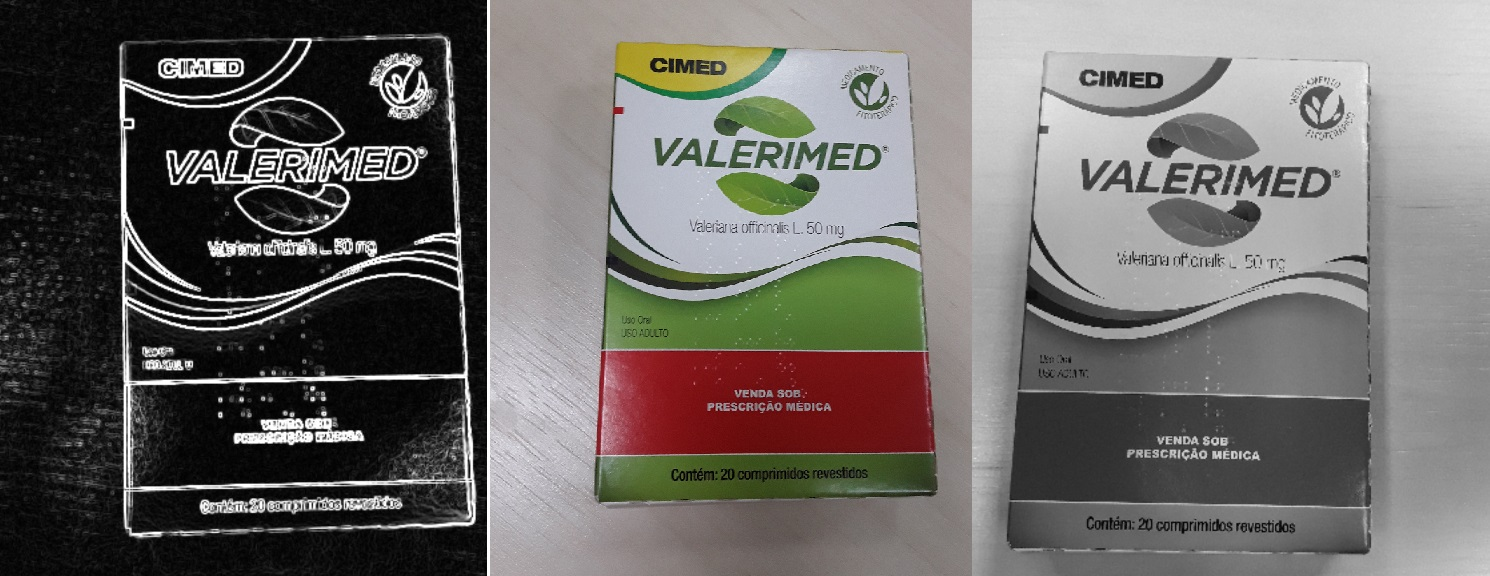
\includegraphics[width=0.90\textwidth]{Imagens/tratamentoimg.jpg} 
	\caption[Imagens expostas ao processamento de imagem.]{Imagens expostas ao processamento de imagem.}
\fonte{Autoria própria.}
	\label{tratamentoimg}
\end{figure}